\section{IrvanRizkiasyah - 1174043}
	\subsection{Data Geospasial}
	Istilah data geospasial dapat juga diganti dengan data spasial atau data GIS (geospatial information system data) yang merupakan sebuah data mengenai aspek fisik dan administratif dari sebuah objek geografis. Aspek fisik di sini mencakup pula bentuk anthropogenic dan bentuk alam baik yang terdapat di permukaan maupun di bawah permukaan bumi. Bentuk anthropogenic mengandung di dalamnya fenomena budaya seperti jalan, rel kereta api, bangunan, jembatan, dan sebagainya. Bentuk alam tentu saja adalah sungai, danau, pantai, daratan tinggi, dan sebagainya. Sedangkan aspek administratif adalah pembagian atau pembatasan sosio-kultural yang dibuat oleh suatu organisasi atau badan untuk keperluan pengaturan dan pemakaian sumberdaya alam.
	
	Sumber dari data geospasial dapat berupa :
	\begin{itemize}
		\item Data sistem penentuan posisi global (GPS). Data GPS dikumpulkan melalui sistem navigasi radio berbasis satelit dan darat. Smartphone berkemampuan GPS dapat memberikan lokasi seseorang.
		\item Data penginderaan jauh, melibatkan sebuah instrumen khusus yang digunakan untuk menangkap data yang bisa diubah menjadi dalam bentuk digital. Pemindai, satelit dan sistem radar merupakan contoh dari instrumen ini. Salah satu contoh dari penginderaan jauh ini adalah foto udara.
	\end{itemize}
	
	Foto udara dapat digunakan untuk mengenali beberapa obyek yang ada di muka bumi. Dengan menganalisa bentuk, ukuran dan warna obyek ini, kita dapat mengamati adanya tanah basah atau kering, tanaman sehat atau tanaman terserang penyakit, serta sawah irigasi atau sawah tadah hujan. Tanah basah akan berwarna lebih gelap bila dibandingkan dengan tanah yang kering.

	\subsection{Link video Data Geospasial}
		\href{https://youtu.be/w1NwuEcDHfA} {Link video Data Geospasial Irvan Rizkiansyah - 1174043}
		
	\subsection{Plagiarism}
	\begin{figure}[H]
		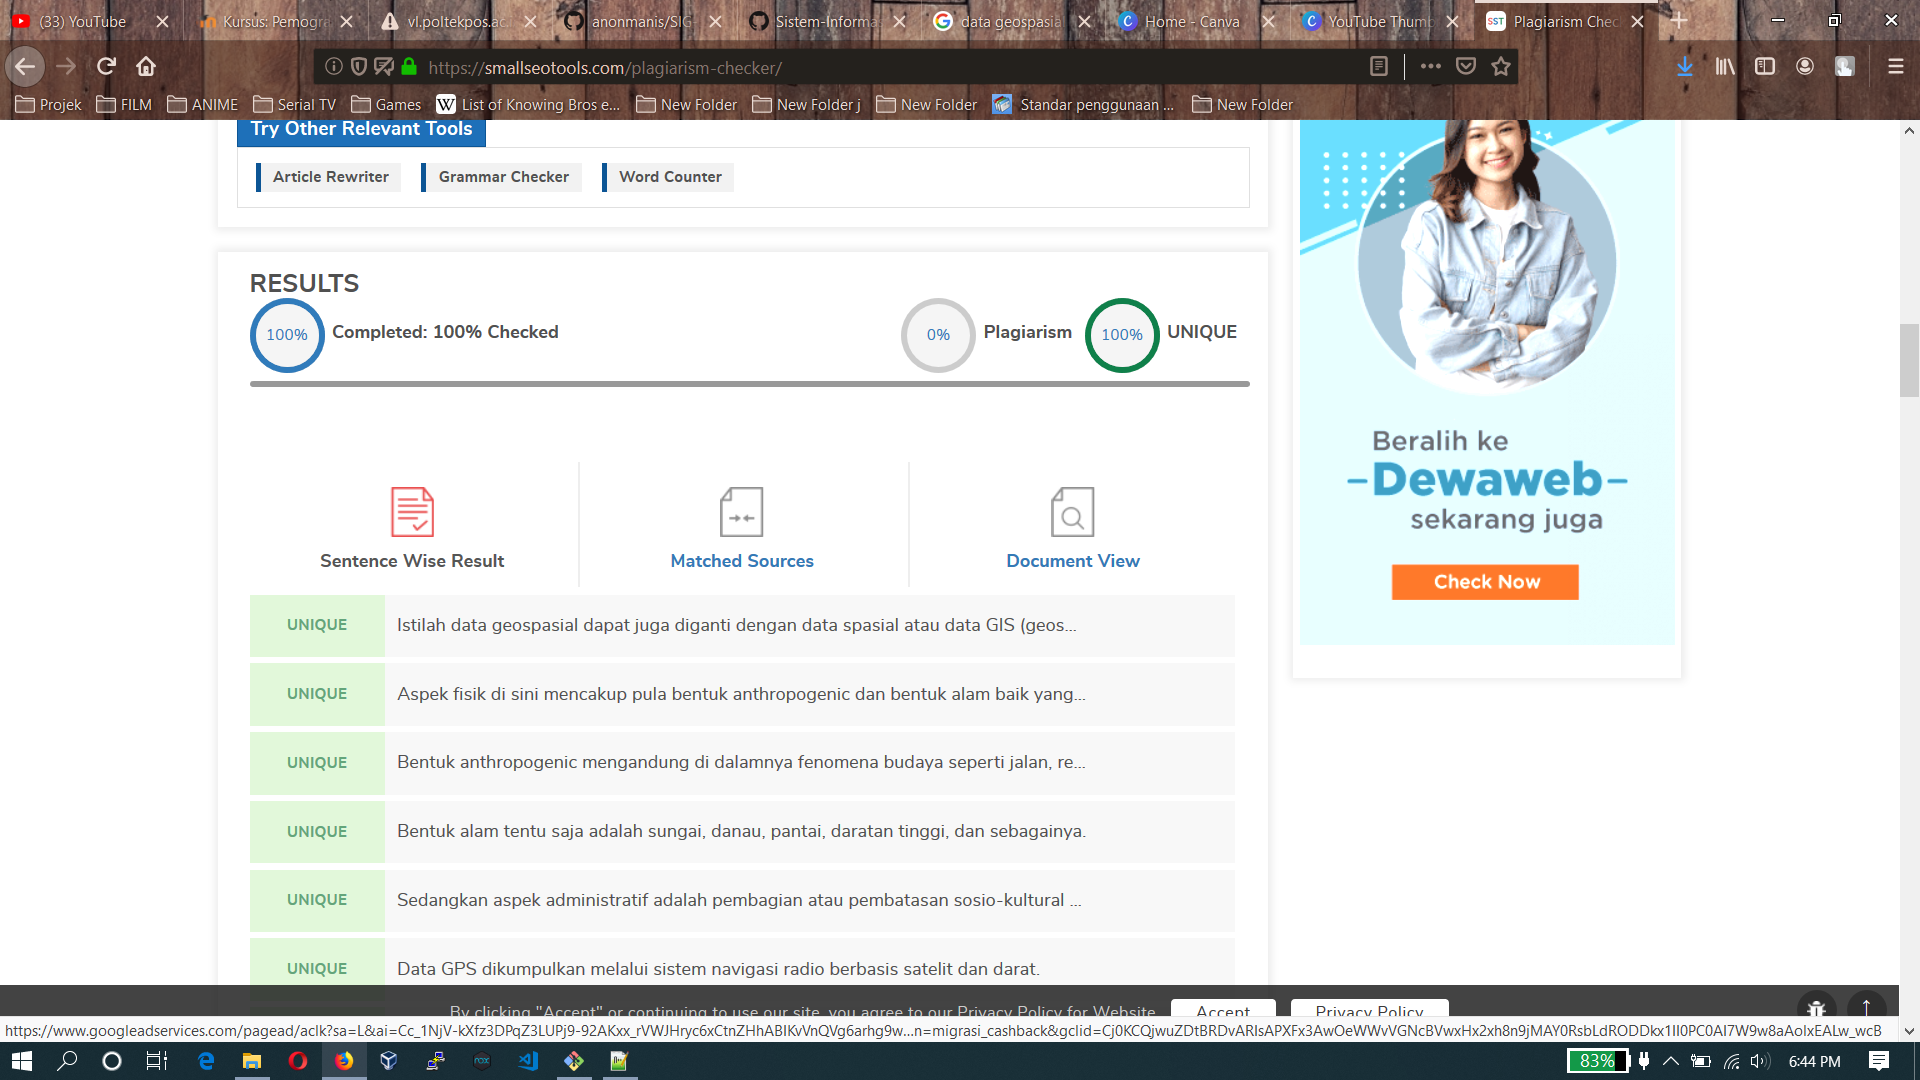
\includegraphics[width=10cm]{figures/1174035/Plagiarisme.png}
		\centering
		\caption{Hasil Pengecekan Plagiarisme}
	\end{figure}